\documentclass[12pt,a4paper]{article}%
\usepackage{amsthm}
\usepackage{amsmath}%
\usepackage{amsfonts}%
\usepackage{amssymb}%
\usepackage{graphicx}
\usepackage[T2A]{fontenc}
\usepackage[utf8]{inputenc}
\usepackage[english,russian]{babel}
%-------------------------------------------
\setlength{\textwidth}{7.0in}
\setlength{\oddsidemargin}{-0.35in}
\setlength{\topmargin}{-0.5in}
\setlength{\textheight}{9.0in}
\setlength{\parindent}{0.3in}

\newtheorem{theorem}{Theorem}
\newtheorem{task}[theorem]{Задача}
\addto\captionsrussian{\renewcommand*{\proofname}{Решение}}


\newcommand{\abovemath}[2]{\ensuremath{\stackrel{\text{#1}}{#2}}}
\newcommand{\aboveeq}[1]{\abovemath{#1}{=}}
\newcommand\bydef{\aboveeq{def}}

\begin{document}
\begin{flushright}
    \textbf{Константин Киреев 8383\\
    \today}
    \end{flushright}
    
    \begin{center}
    \textbf{Формальные языки\\
    HW01} \\
    \end{center}
    \task{Привести грамматику для языка $\{\alpha \cdot abbab \cdot \beta | \alpha, \beta \in \{a, b\}^*\}$. Привести вывод и дерево вывода для 2 различных цепочек из языка.}
    \begin{proof}
        \begin{align*}            
            &G = \langle V_T, V_N, P, S \rangle \\
            &V_T = \{a, b\} \\
            &V_N = \{S, A, B\}
        \end{align*}
        \begin{align*}  
            P = \{&S\rightarrow A \\ 
            &A \rightarrow aA | abbabB \\
            &B \rightarrow bB | A | \epsilon \} 
        \end{align*}
        
        \begin{itemize}
            \item $aaabbabb = S\rightarrow A \rightarrow aA\rightarrow aaA\rightarrow aaabbabB\rightarrow aaabbabbB\rightarrow aaabbabb\epsilon\rightarrow aaabbabb$
            \item $abbab = S\rightarrow A\rightarrow abbabB \rightarrow abbab\epsilon\rightarrow abbab$
        \end{itemize}
        \begin{figure}[h!]
            \center{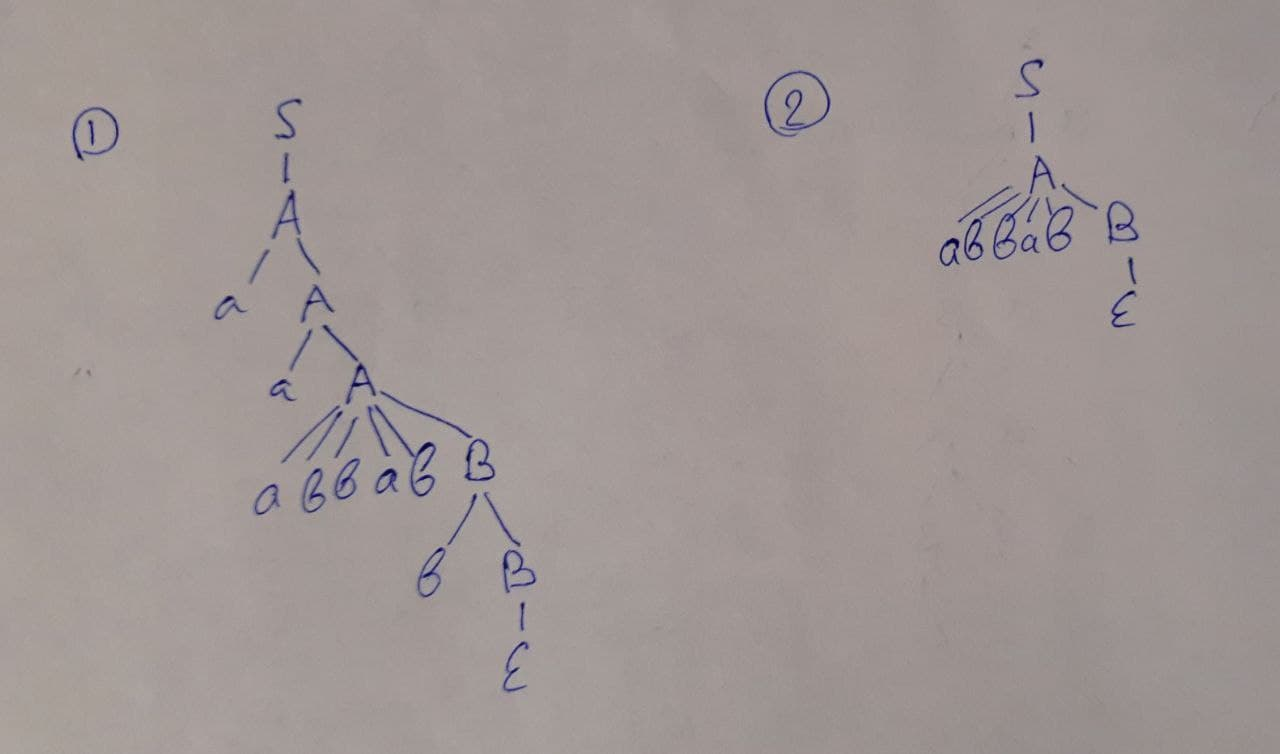
\includegraphics[scale=0.35]{1.jpg}}
        \end{figure}
    \end{proof}   
    \task{Доказать или опроыергнуть, что для любых языков $L$ и $M$ верно $(L\cdot M)^r = M^r \cdot L^r$}
    \begin{proof}
        -
    \end{proof}

    \task{Перечислить все слова языка $\{c^na^nt^n | n \in \mathbb{N}_0 \} \cap \{(cat)^m | m \in \mathbb{N}_0\}$}
    \begin{proof}
        $ $
        \begin{itemize}
            \item cat
            \item $\epsilon$
        \end{itemize}
    \end{proof}
\end{document}